\documentclass[12pt,a4paper]{report}
\usepackage[utf8]{inputenc}
\usepackage{graphicx}
\usepackage{hyperref}
\usepackage{geometry}
\usepackage{booktabs}
\usepackage{titlesec}

\geometry{a4paper, margin=1in}

\titleformat{\chapter}[display]
  {\normalfont\huge\bfseries}{\chaptertitlename\ \thechapter}{20pt}{\Huge}
\titlespacing*{\chapter}{0pt}{50pt}{40pt}

\begin{document}

\begin{titlepage}
    \centering
    \vspace*{2cm}
    
    {\Large Software Engineering Project Report \par}
    \vspace{1.5cm}
    
    {\Huge\bfseries MathVerse AI \par}
    \vspace{0.5cm}
    {\Large \textit{A Gamified, AI-Powered Mathematics Learning Platform} \par}
    
    \vspace{3cm}
    
    {\Large \textbf{Submitted by:} \par}
    Your Name (Roll Number) \par
    Team Member 2 (Roll Number) \par
    \vspace{1.5cm}
    
    {\Large \textbf{Submitted to:} \par}
    Professor / Evaluator Name \par
    
    \vfill
    
    {\Large \textbf{Computer Science and Engineering Department} \par}
    {\Large Thapar Institute of Engineering and Technology, Patiala \par}
    \vspace{1cm}
    
    {\large \today \par}
\end{titlepage}

\tableofcontents
\newpage

\chapter{Introduction}

\section{Background and Context}
Mathematics anxiety and a lack of student engagement are pervasive challenges in modern education. Traditional pedagogical methods often fail to motivate students or adapt to their individual learning paces. Gamification—integrating game mechanics such as points, leaderboards, and narratives into non-game environments—has shown significant promise in improving educational outcomes. Furthermore, the advent of generative artificial intelligence (AI) provides an unprecedented opportunity to offer personalized, real-time tutoring. 

MathVerse AI is an immersive, gamified learning platform that combines superhero-themed narrative elements (such as "Boss Battles" and "Missions") with adaptive AI tutoring. By transforming math problems into interactive quests, MathVerse AI aims to sustain student engagement while providing verifiable academic progress.

\subsection{Problem Statement}
Current e-learning platforms typically fail in two areas: they either rely on static question banks that encourage rote memorization without building deep conceptual understanding, or they lack the intrinsic motivational hooks necessary to keep students engaged over long periods. Administrators and educators also lack granular insights into where a student is struggling. MathVerse AI addresses this by (a) dynamically generating context-aware math problems using AI, (b) wrapping the learning experience in a compelling superhero narrative with virtual rewards, and (c) providing robust analytics for performance tracking.

\section{Project Objectives}
\begin{enumerate}
    \item \textbf{Objective 1:} Design and implement a robust relational data model (using PostgreSQL) to track user progress, virtual wallets (Spider Points), mission completion statuses, and gamification metrics.
    \item \textbf{Objective 2:} Build a responsive, modern web application frontend using React and Vite, featuring rich animations and a highly engaging, theme-driven user interface.
    \item \textbf{Objective 3:} Develop a secure, stateless REST API backend that integrates seamlessly with AI models to dynamically generate adaptive mathematics challenges based on the user's skill level.
    \item \textbf{Objective 4:} Implement core gamification business logic, including atomic transactions for virtual currency rewards, leaderboard ranking, and stateful tracking of "Boss Battles."
\end{enumerate}

\chapter{Methodology and Design}

\section{System Architecture}
MathVerse AI follows a modern three-tier web architecture: a dynamic React single-page application (SPA), a stateless backend API (Python/Node.js), and a relational database, heavily augmented by an external AI Layer.

\subsection{High-Level Design}
The frontend acts as the primary interface for students, featuring dashboards, mission selection screens, and interactive boss battle arenas. It communicates asynchronously with the backend API. The system enforces role-based access control, ensuring that students can only access their specific missions, while teachers and parents have access to learning reports.

\section{System Design Diagrams}

\subsection{Use Case Diagram}
The system serves three primary actors: the \textbf{Student}, \textbf{Teacher}, and \textbf{Parent}. Students can login, play math missions, and track their progress. During missions, the system evaluates their answers and provides optional hints via the AI tutor (Gwen). Teachers and parents can monitor progress through dedicated learning reports.

\vspace{0.5cm}
\begin{figure}[h]
    \centering
    % Ensure you save the provided Use Case Diagram image as 'use_case.png' in an 'assets' folder
    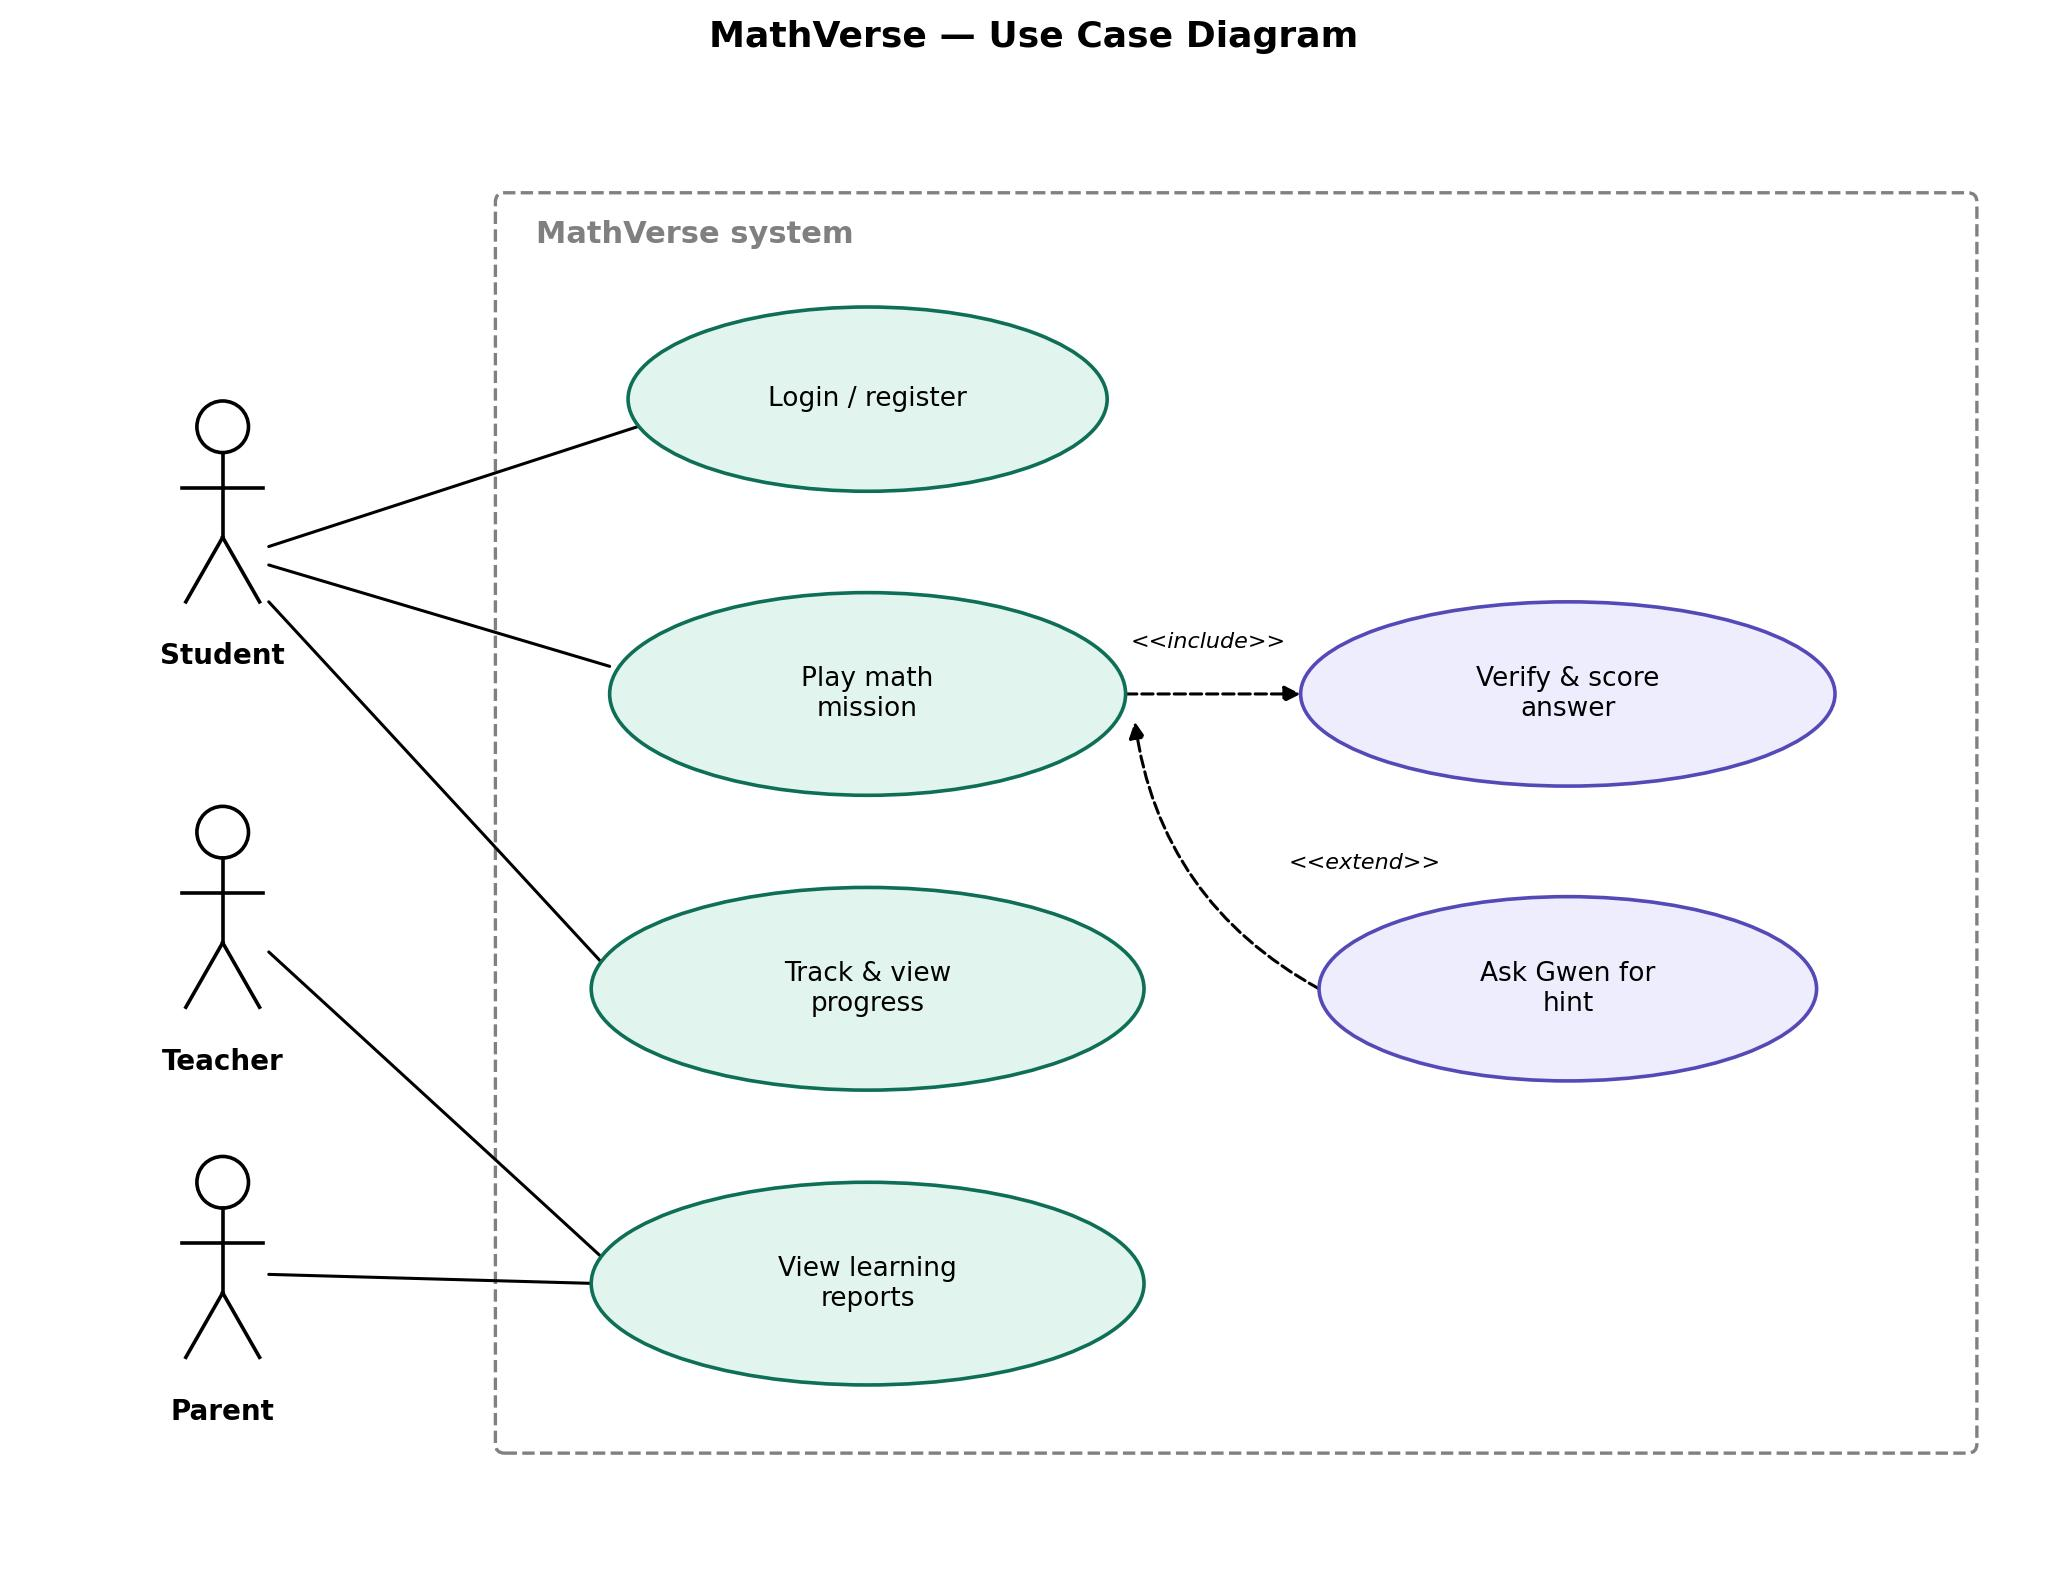
\includegraphics[width=0.9\textwidth]{assets/use_case.png}
    \caption{MathVerse Use Case Diagram}
\end{figure}
\vspace{0.5cm}

\subsection{Sequence Diagram (Mission Run)}
The sequence diagram illustrates the lifecycle of a mission run. The student requests a mission through the frontend, which calls the backend. The backend retrieves the appropriate questions from the database and returns them. Upon submission, the backend verifies the answer, updates mastery scores, and asynchronously triggers the AI layer to analyze behavior and predict risk.

\vspace{0.5cm}
\begin{figure}[h]
    \centering
    % Ensure you save the provided Sequence Diagram image as 'sequence.png' in an 'assets' folder
    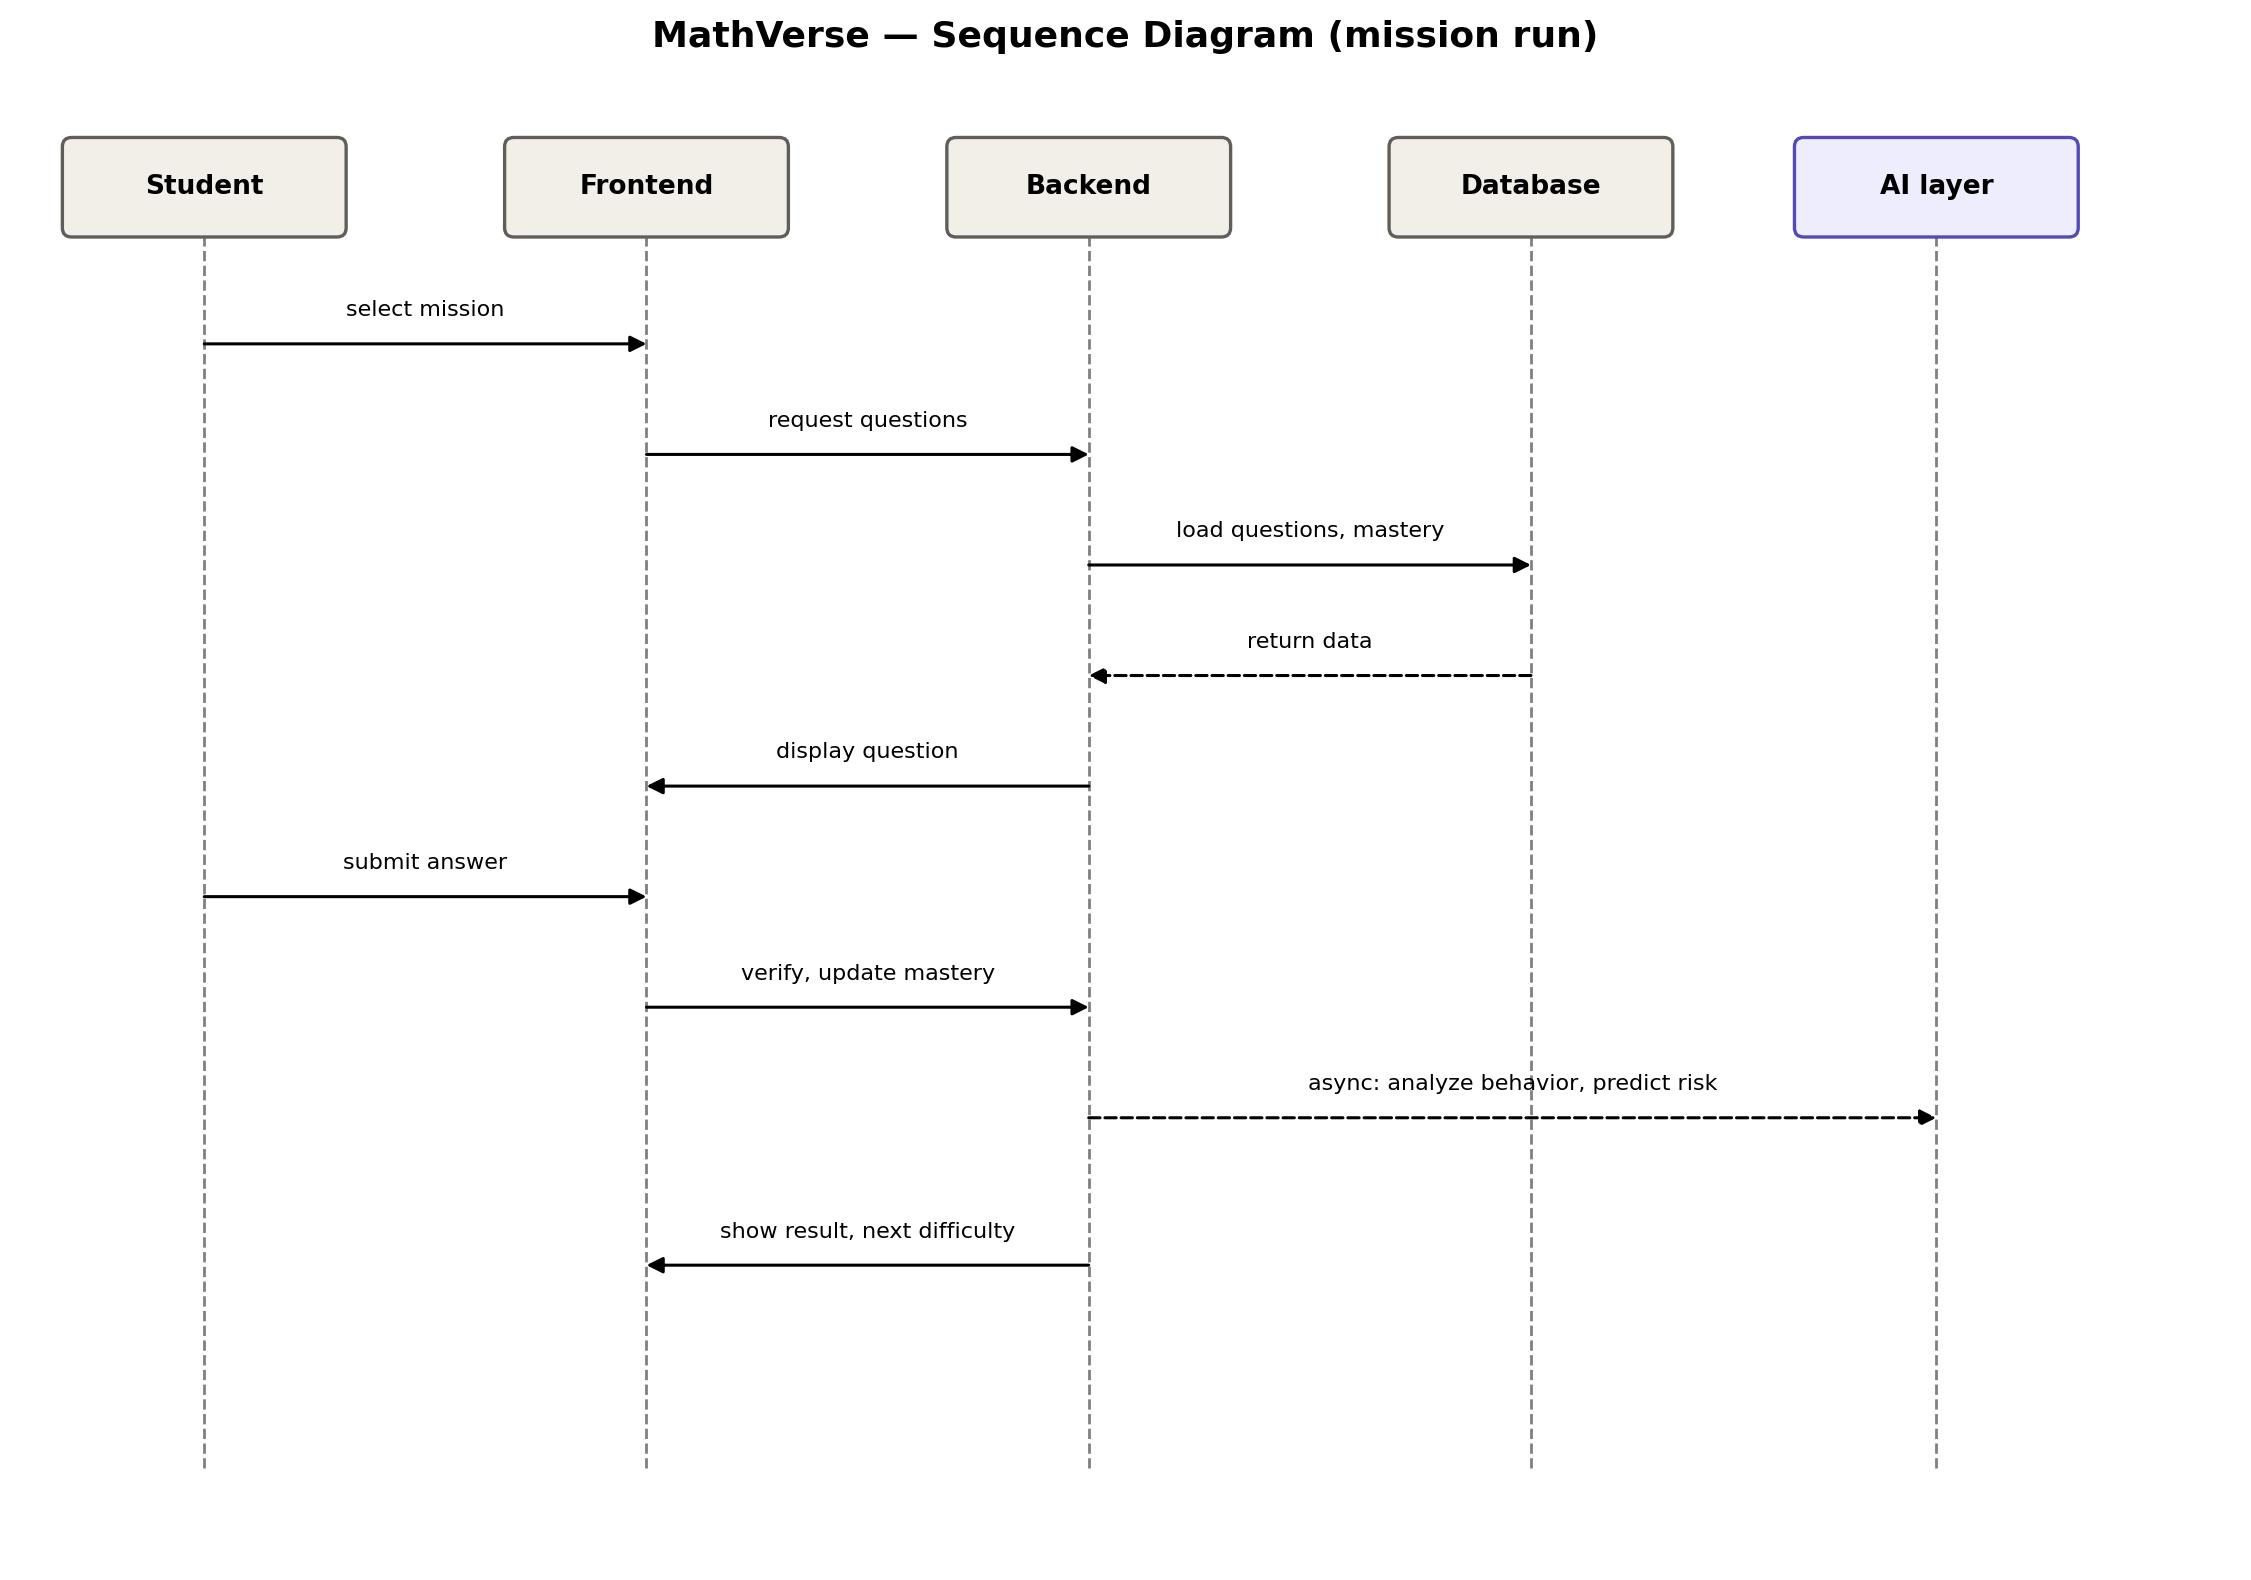
\includegraphics[width=0.9\textwidth]{assets/sequence.png}
    \caption{MathVerse Sequence Diagram for a Mission Run}
\end{figure}
\vspace{0.5cm}

\subsection{Activity Diagram (Student Journey)}
The student journey maps out the logical flow of a user navigating the system: logging in, selecting a mission, solving questions, and receiving system-level verification and AI-level analysis (non-blocking). It culminates in updating progress badges and generating reports.

\vspace{0.5cm}
\begin{figure}[h]
    \centering
    % Ensure you save the provided Activity Diagram image as 'activity.png' in an 'assets' folder
    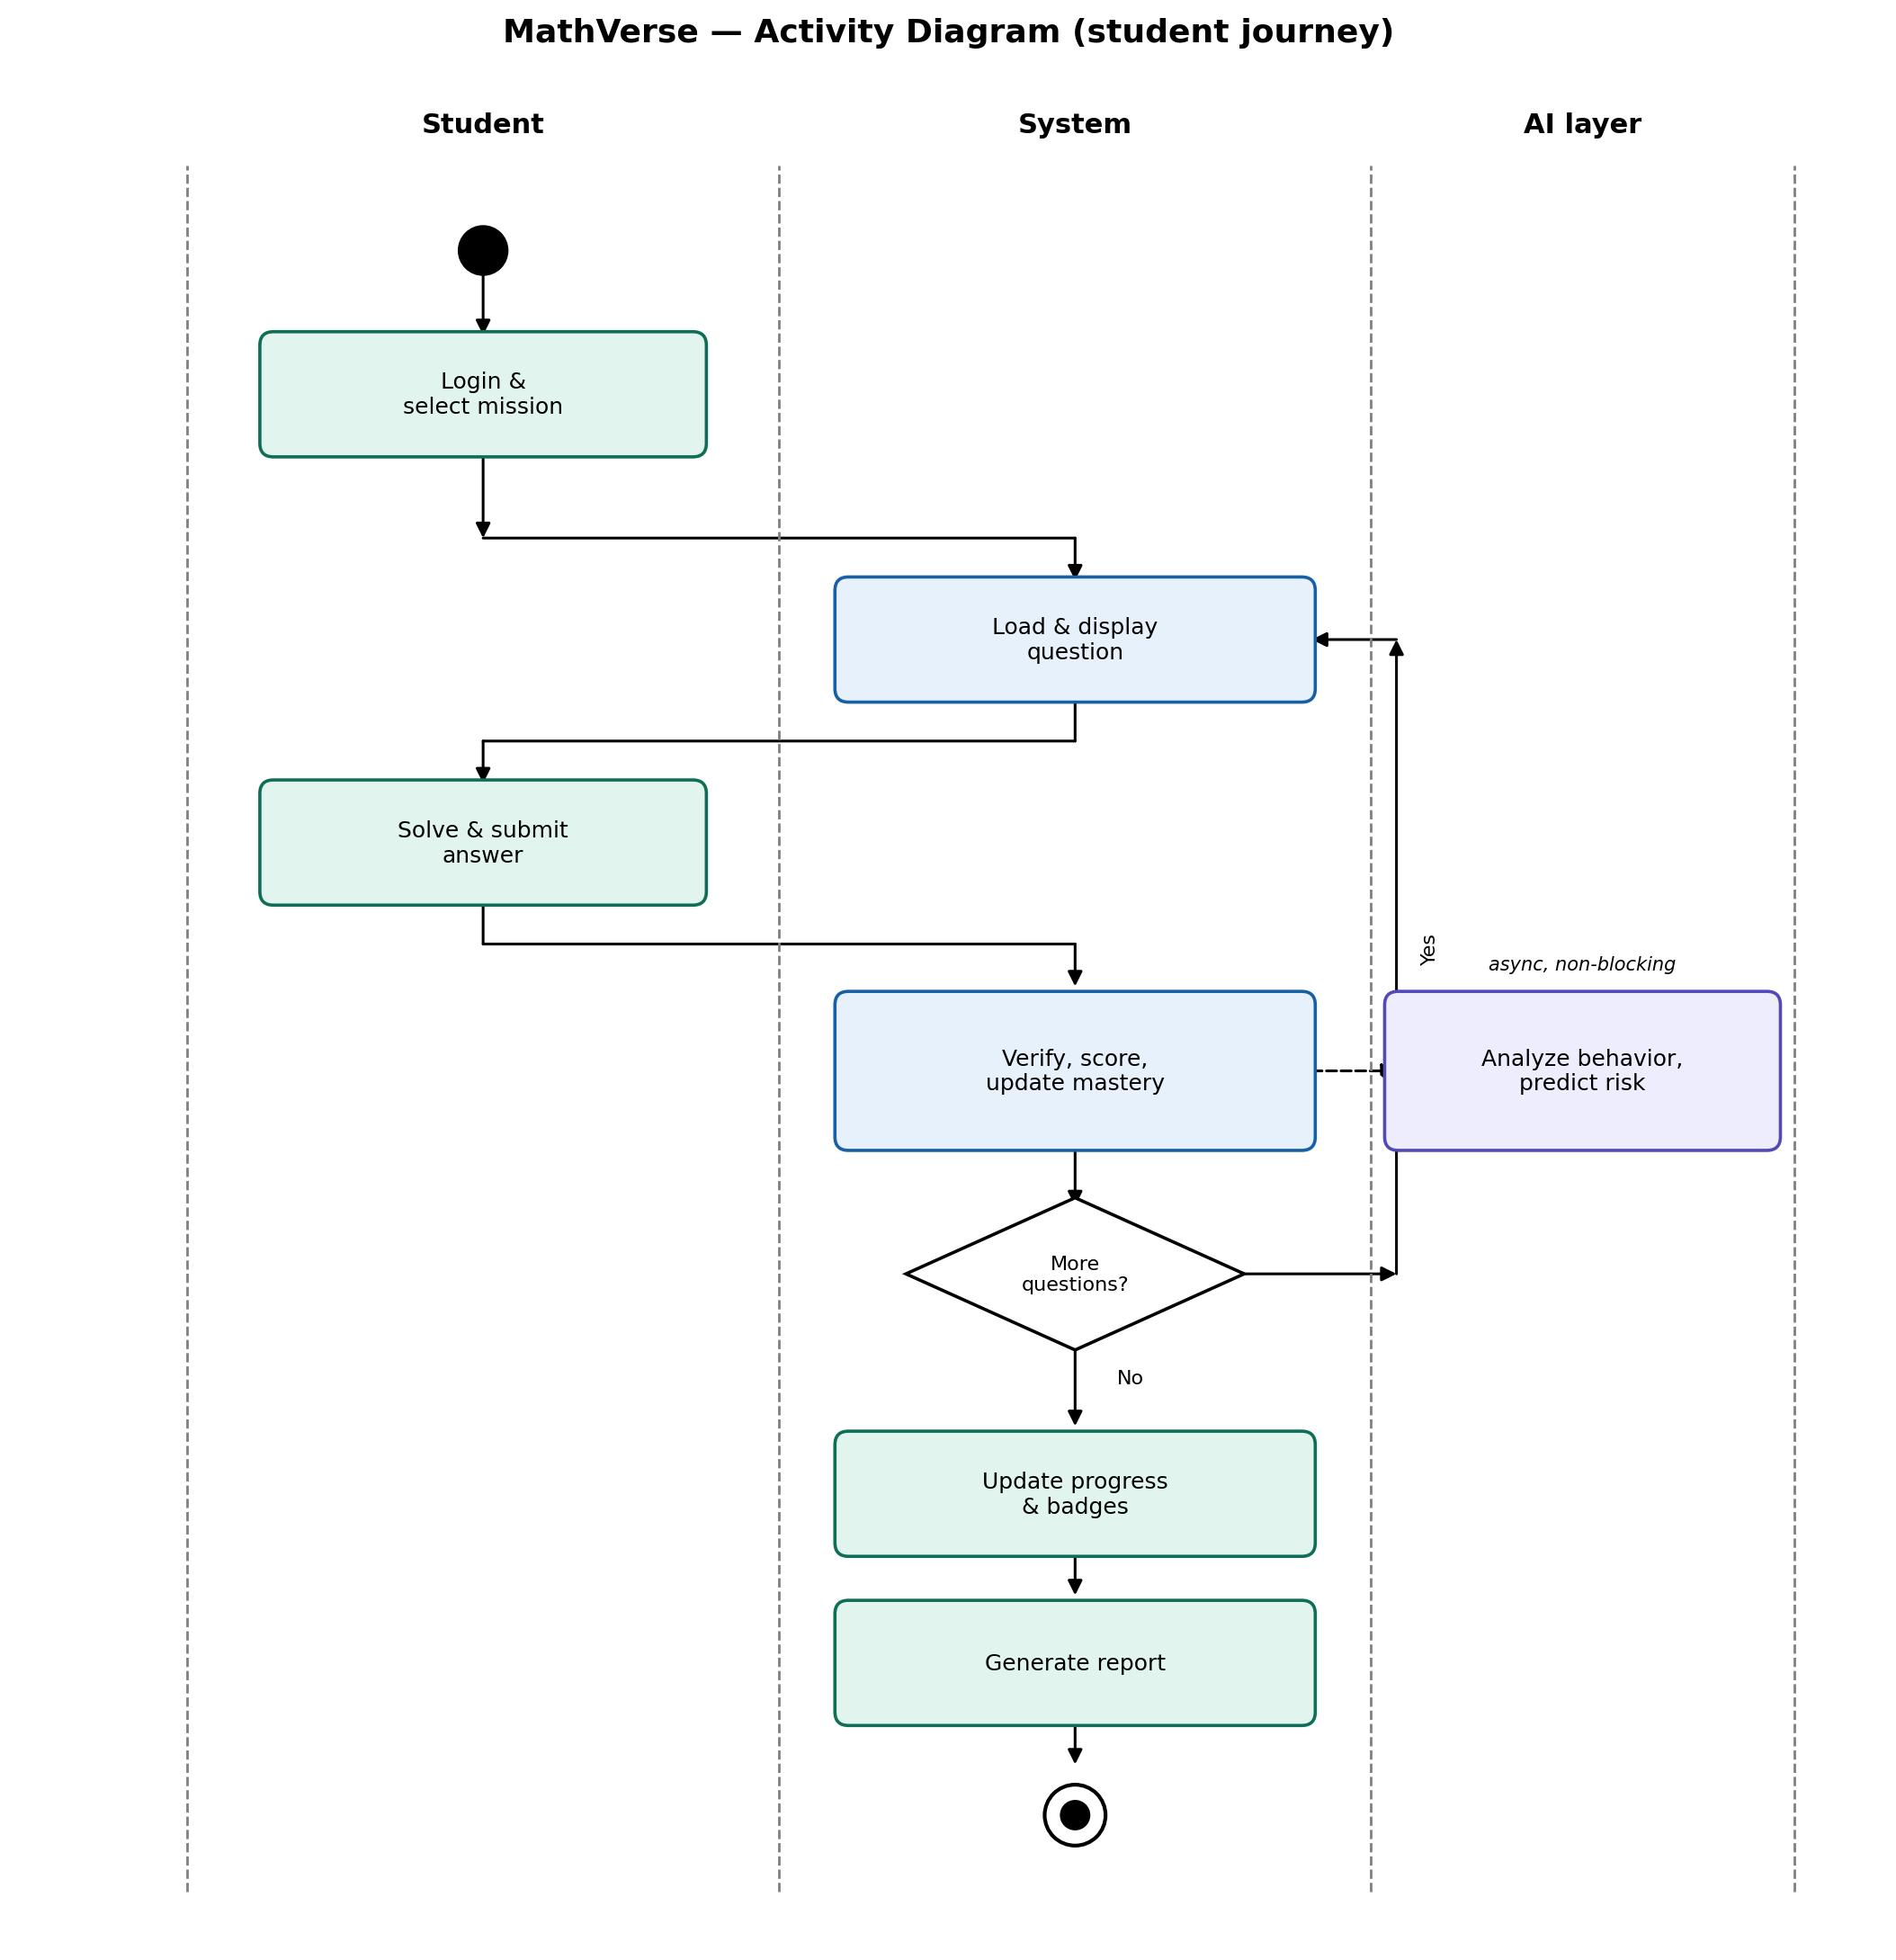
\includegraphics[width=0.9\textwidth]{assets/activity.png}
    \caption{MathVerse Activity Diagram depicting the Student Journey}
\end{figure}
\vspace{0.5cm}

\subsection{Class Diagram}
The Class Diagram outlines the domain models, separating the core educational elements (\texttt{Student}, \texttt{Mission}, \texttt{MissionAttempt}, \texttt{Progress}, \texttt{Badge}) from the advanced AI features (\texttt{RAGTutor}, \texttt{LSTMPredictor}). This illustrates a clean separation of concerns where the educational models feed data into the AI layer.

\vspace{0.5cm}
\begin{figure}[h]
    \centering
    % Ensure you save the provided Class Diagram image as 'class.png' in an 'assets' folder
    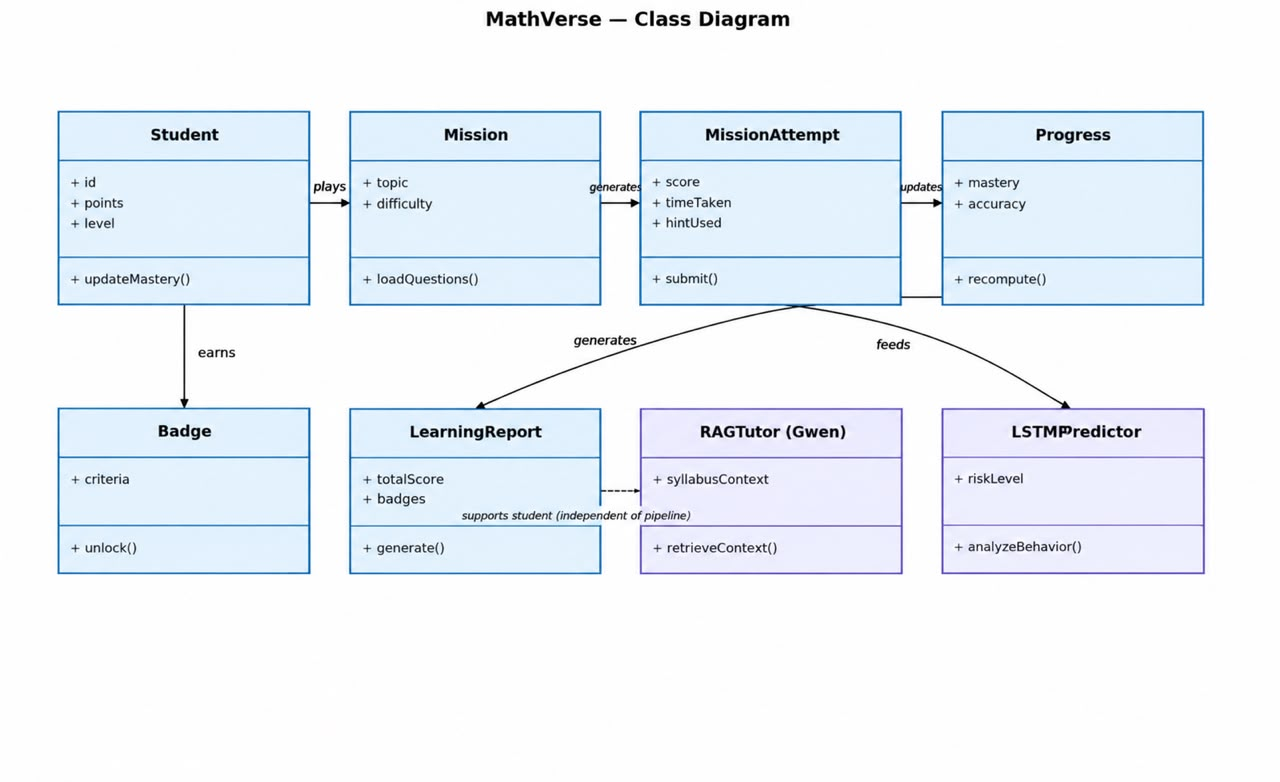
\includegraphics[width=0.9\textwidth]{assets/class.png}
    \caption{MathVerse Class Diagram}
\end{figure}
\vspace{0.5cm}

\section{Implementation Details}
\textbf{Adaptive AI Problem Generation:}
The integration of LLMs for generating math problems utilizes strict prompt engineering to maintain educational standards and thematic consistency. The AI service constructs prompts with explicit constraints, specifying the grade level, the mathematical concept (e.g., linear equations), and the superhero narrative wrapper.

\textbf{Transactional Gamification Economy:}
Managing the distribution of "Spider Points" required robust transactional integrity to prevent race conditions or duplicate awards during rapid network requests. When a student successfully completes a Boss Battle, the GamificationService initiates an atomic database transaction.

\chapter{Results and Evaluation}

\section{Testing Methodology}
Verification of MathVerse AI utilized a combination of manual functional testing and automated integration tests. Functional testing ensured that all core routes (authentication, mission submission, wallet updates) performed as expected. Integration testing verified that the frontend dashboard correctly reflected the database states.

\section{System Verification}

\begin{table}[h]
\centering
\begin{tabular}{@{}p{3.5cm}p{8.5cm}l@{}}
\toprule
\textbf{Flow} & \textbf{Verified Behaviour} & \textbf{Result} \\ \midrule
Registration \& Login & New user receives a default wallet balance. Incorrect credentials are rejected. & Pass \\ 
Mission Submission & Correct answers securely trigger a transactional wallet update and mission completion flag. & Pass \\ 
Boss Battles & Health points are dynamically reduced based on answer accuracy and speed. & Pass \\ 
Role-gated Routes & Students are denied access to admin-only analytics endpoints with a 403 Forbidden status. & Pass \\ \bottomrule
\end{tabular}
\caption{Summary of functional verification against the backend}
\end{table}

\section{Analysis}
The implementation successfully met the core objectives outlined in Chapter 1. The robust data model effectively supports the gamified economy, and the React frontend provides the highly interactive experience required for student engagement. 

\chapter{Conclusion}

\section{Summary of Work}
This report detailed the design and implementation of MathVerse AI, a gamified platform designed to enhance mathematics education. The current phase focused extensively on establishing the high-fidelity React frontend and designing the overarching system architecture.

\section{Future Scope and Next Steps}
As outlined in the system design diagrams, the immediate future scope is focused purely on executing and completing the backend and AI integrations detailed in our architectural models. The roadmap includes:
\begin{enumerate}
    \item \textbf{Implementation of RAGTutor (Gwen):} Integrating a Retrieval-Augmented Generation (RAG) tutor to provide real-time, context-aware hints independently of the main evaluation pipeline.
    \item \textbf{LSTM Risk Predictor Integration:} Deploying the \texttt{LSTMPredictor} module to asynchronously analyze student behavior during missions and predict learning risks without blocking the UI.
    \item \textbf{Teacher and Parent Portals:} Building out the frontend views and secure endpoints for Teachers and Parents to access the \texttt{LearningReports} generated from student progress.
    \item \textbf{Full Backend Synchronization:} Finalizing the database connections for \texttt{MissionAttempt} logging and real-time mastery updates as dictated by the Sequence Diagram.
\end{enumerate}

\section{Final Remarks}
MathVerse AI demonstrates the powerful potential of combining educational technology with game design and artificial intelligence. The foundation built during this project provides a highly scalable and extensible platform that can fundamentally change how students interact with and learn mathematics.

\end{document}
